%\documentclass[11pt]{article}
\documentclass{article} % For LaTeX2e
\usepackage{nips13submit_e,times}
\usepackage{hyperref}

\usepackage{graphicx}
\usepackage{epsfig}
\usepackage{caption}
\usepackage{subcaption}
\usepackage{cite}
\usepackage{url}
\usepackage{wrapfig}



\newcommand{\fix}{\marginpar{FIX}}
\newcommand{\new}{\marginpar{NEW}}

%\nipsfinaltrue  % Uncomment for camera-ready version

\begin{document}

\title{Unsupervised learning of the connections  \\ between layers of deep neural networks}

\author{
Eugenio Culurciello\thanks{More information on Eugenio Culurciello's laboratory and research can be found here: http://engineering.purdue.edu/elab/. Real time robotic vision systems: http://www.neuflow.org/} \\
Purdue University\\
\texttt{euge@purdue.edu} \\
\And
Aysegul Dundar \\
Purdue University\\
\texttt{adundar@purdue.edu}
\AND
Jonghoon Jin \\
Purdue University\\
\texttt{jhjin@purdue.edu}
\And
Jordan Bates \\
Purdue University\\
\texttt{jtbates@purdue.edu}
}

%\date{\today}

\maketitle

\begin{abstract}
We present the unsupervised clustering learning technique for learning the connection matrix between layers of a deep neural networks. Traditional deep neural networks use random connection tables between layers to keep the number of  connection small and tune to different image features. Fully-connected layers are also used when efficiency is not an issue. These kind of connections perform adequately in supervised deep networks because the training refines their values. 
On the other hand, unsupervised learning requires a data-driven method that will connect the most relevant features to the next layer. In this paper we present a clustering learning algorithm to learn simultaneously the connection and filters of deep networks. We tested our technique on CIFAR, SVHN and Pedestrian datasets and improve the accuracy by ?? compared to ... We show that networks and connections trained with clustering learning can obtain similar levels of performance as supervised deep networks when the number of layers and the filters are the same. 
This work can be applied to improve the efficiency of connections and combination of features between the layers of deep neural networks.
\end{abstract}


\section{Introduction}

Most scientists and engineers are fascinated by the design of an artificial vision system that can reproduce some of the human visual system capabilities in detecting, categorizing, tracking objects in view. The availability of a real-time synthetic vision system with such capabilities would find use in a large variety of applications, such as: autonomous cars, co-robots helpers, smart appliances, cellular-phones, to name a few. The most promising approach in recent years, is the fusion of bio-inspired and neuromorphic vision models with machine learning \cite{lecun_gradient-based_1998,hadsell_dimensionality_2006,gregor_structured_2011,riesenhuber_hierarchical_1999,serre_feedforward_2007,serre_neuromorphic_2010,jarrett_what_2009,lecun_convolutional_2010,boureau_theoretical_2010}. This field, named Deep Learning, has provided state-of-the-art results in the categorization of multiple objects in static frames \cite{krizhevsky_imagenet_2012}.

Deep Learning networks are computer-vision and computational-neuroscience models of the mammalian visual system implemented in deep neural networks, where each network layer is composed of: linear two-dimensional filtering, non-linearity, pooling of data, output data normalization \cite{jarrett_what_2009,lecun_convolutional_2010,boureau_theoretical_2010}. 
Deep Networks training is performed by means of the abundant image frames and videos one can find on the internet and large labeled datasets. In particular, deep networks need to learn good feature representations for complex visual tasks such as object categorization and tracking of objects in space and time, identifying object presence and absence. These representations usually involve learning the linear filter weight values from labeled and unlabeled input data. Since labeled data is costly and often ridden with human errors \cite{karpathy_lessons_2011, torralba_unbiased_2011, hou_meta-theory_2012}, the recent focus is on learning these features purely from unlabeled input data \cite{olshausen_emergence_1996, hyvarinen_independent_2000, hinton_fast_2006, vincent_extracting_2008, coates_analysis_2011}. These recent methods typically learn multiple layers of deep networks by training several layers of features, one layer at a time, with varying complexity of learning models. Traditional work in unsupervised deep learning has focused on learning layer features, and rarely on the connections between layers. In this paper we present unsupervised clustering algorithms applied to learning the connectivity matrix between layers and filters of deep neural networks for general-purpose vision systems. 

Recent techniques based on unsupervised Clustering Learning (Cl) are especially promising because they use simple learning methods that quickly converge \cite{culurciello2013clustering,coates_analysis_2011}. 
These algorithms are easy to setup and train and are especially suited for applied research, because environment-specific data can be collected quickly with a few minutes of video, setup of custom size deep networks is quick and can be adapted to specific tasks in minutes.

The paper presents the following key innovations: (1) use of clustering learning for learning both filters and connections of deep networks with fully unsupervised techniques (Section \ref{sec-main}), (2) the ability to self-organize connections and filters purely with a data-driven approach from video streams (Section \ref{sec-methods} and  \ref{sec-net-arch}), (3) the ability of trained network to perform as well as supervised networks trained on still frames (Section \ref{sec-results}), (4) the ability to run in real-time due to a optimized lean network with 32 filters or less in the first, most computationally expensive network layer (Section \ref{sec-net-arch}). 



\section{Main idea and contribution}
\label{sec-main}

The connections between layers in a deep neural network are a very important parameter. It has been shown that in many cases random filters perform only slightly worse than fully trained network layers \cite{saxe2011random} suggesting that filters, used in the convolutional module of each layer, might not play a dominant role in determining the network performance.
Rather, the connections between layers and the combination of features are mainly responsible for the recent success of supervised deep convolutional networks \cite{krizhevsky_imagenet_2012}. In these networks the connection between layers is learned from the data using global gradient-descent techniques at large scale. Because training will intimately select the strength of connections, developers of deep networks have traditionally used fully connected layers, custom table connections \cite{lecun_gradient-based_1998}, or random connections \cite{lecun_convolutional_2010}. The reason for using custom connection matrices is to reduce the number of computations, and avoid over fitting problems.
 
In unsupervised deep networks, one cannot rely on back-propagation techniques to learn the connections between layers. This is because unsupervised networks do not used labeled data, and thus an error signal cannot be computed. Fully connected layers can be used \cite{culurciello2013clustering,coates_analysis_2011} at the expense of more computational time and also reduced performance. The lower performance is attributable to the averaging effect that a fully connected layer has in unsupervised network, where the strengths of connection is not adapted to the training data. In order to use unlabeled data to train large deep networks, we investigate different techniques of grouping features from one layer into features of the next layers, and at the same time learn the filters needed by the next layer. A figure that qualitatively explains the main contribution of the paper is Fig. \ref{fig-learnlayers}.

\begin{figure}
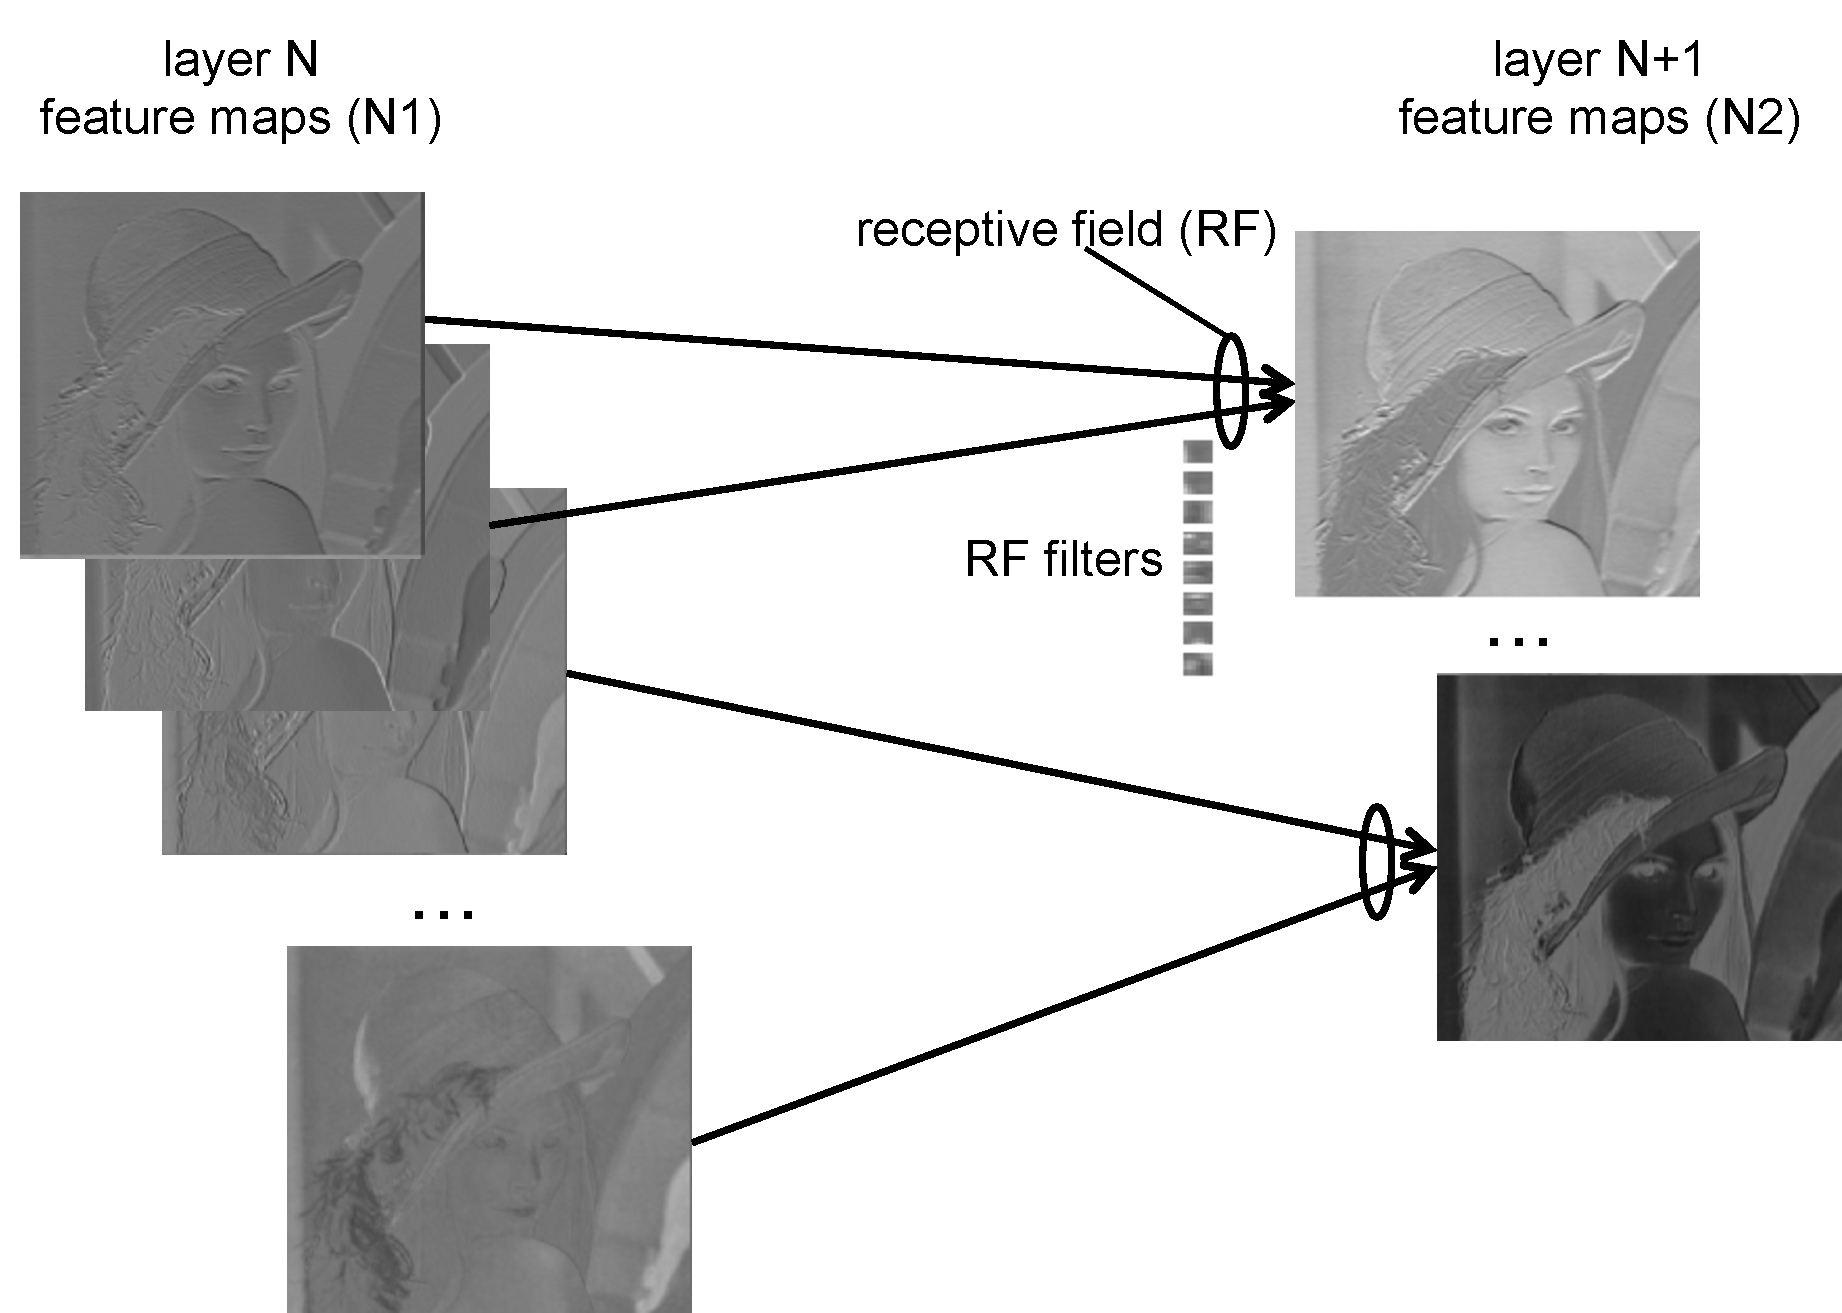
\includegraphics[width=5in]{fig-learnlayers.pdf}
\caption{Learn layers}
\label{fig-learnlayers}
\end{figure}


In the figure we show two layers of a deep network: layer $N$ and layer $N+1$. The maps on the left of the figure, are the $N1$ output feature maps of the $N$-the layer in response to an input image. The maps on the right of the figure, are the $N2$ outputs of the first convolutional module of layer $N+1$. 

We investigate different techniques of grouping feature maps from layer $N$ into "receptive fields" (RF). These receptive fields are the input of one or multiple maps in layer $N+1$. We form these RF by 4 different methods. 1) Grouping a small number of layer $N$ features that co-occur in one or multiple sets of feature maps from layer $N$. In other words, we look for features that are highly activated in the same pixel, and we group these features into the RF. In Fig. \ref{fig-learnlayers}, these are $G$ groups of $K$ maps. The idea behind this step is to group features that occur often together in the data. 2) Selecting a small number of layer $N$ features randomly, 3) Grouping each maps individually, in other words if there are 32 filters in the first layer and so 32 maps are created after the first layer, we create 32 groups each has only 1 map, and 4) Grouping all maps into 1 group. 
In order to learn the filters for layer $N+1$ convolutional module, we perform clustering (Clustering Learning) only within the RF (and not all $N1$ maps). In Fig. \ref{fig-learnlayers}, we learn $N2$ filters per group for a total of $N2 \cdot G$ maps in layer $N+1$.

%The main driving force for this idea is a bio-inspired model of learning in the mammalian brain. It is widely believed that one of the possible physical mechanism of learning in the brain is the Hebbian method \cite{masquelier2007learning}. This learning method suggests that a group of pre-synaptic neurons is strongly connected to a post-synaptic neuron if the group (or receptive field, RF) can predict the response of the post-synaptic neuron. In other words neuron in the RF have strong connections to a neuron in layer $N+1$ if they can predict its response. The main contribution of this paper is a real-valued implementation of this learning rule. The RF group features that are highly activated together in the same location. This group of highly activated features will then propagate a high value to the same location in the relative map of layer $N+1$. This implements the Hebbian rule. We call this connection matrix algorithm 'CL-connex'.

In the literature, we found two deep learning papers that are related. 
Paper \cite{coates2012learning} groups features on each layer by similarity, but does not explicitly use connection matrices between layers, rather they flatten the data at each layer and re-apply clustering algorithms. This approach is equivalent to forming a full-connection between layers, which is less efficient because each feature is averaged with a large number of other features, thus reducing the signal-to-noise ratio of important features. 
%The main difference between paper \cite{coates2012learning} and our work is that we focus on learning smaller networks, with much fewer number of filters (32 vs. 4096) in the first and successive layers. 
The paper \cite{boureau_2011} presents the interesting idea of learning pooling strategies that include feature maps with similarity in local feature space. This paper uses simple clustering procedures to cluster data in order to improve pooling in the feature space. In this respect this paper present similar ideas to the first technique we test in this paper, but is not applied to deep neural networks.

%Several papers in the neural physiology and computational neuroscience literature report similar ideas for learning the receptive fields of complex cells \cite{masquelier2007learning,spratling2005learning,wiskott2002slow,wallis1997invariant}. None of these paper reports results close to the state-of-the-art in publicly available datasets of natural images.


\section{Methods}
\label{sec-methods}


We used the Torch7 software for all our experiments \cite{collobert_torch7_2011}, since this software can reduce training and learning of deep networks by 5-10 times compared to similar Matlab and Python tools. In addition it features a "Spatial" mode that allows a trained network to be efficiently applied to any size image, for quick demonstrations and applications.


\subsection{Input data}

We tested and obtained results using the CIFAR10 \cite{krizhevsky_learning_2009} and the Street View House Numbers (SVHN) \cite{netzer_reading_2011} datasets. The SVHN dataset has a training size of 73,257 32x32 images and test size of 26,032 32x32 images. The CIFAR10 dataset has a training size of 20,000 32x32 images and a test size of 2,000 32x32 images. Both datasets offer a 10 categories classification task on 32x32 size images. The train dataset was in all cases learned to 100\% accuracy, and training was then stopped. 

%We also use the INRIA Person Dataset \cite{INRIAperson} to train a person detector. This datasets consists of a training set of of 2416 with size of 96 by 160 pixels, and a test set with 1126 images of 70 by 134 pixels. From this dataset we extracted a 46 by 46 pixels window centered on the torso of each person. We used backgrounds from a youTube video file as background category.
%We trained a 3-layer CL network with CL-connex between layer 1-2 and 2-3.

We did not use the YUV color space in CIFAR10 and SVHN because they were reporting $\sim 2-4\%$ loss in accuracy. This is contrary to what has been reported by others \cite{jarrett_what_2009}. We kept the images of CIFAR10 and SVHN in their original RGB format. Input data was first normalized by subtracting out the mean and dividing by the standard deviation and then whitened.
%The YUV format was used in the INRIA person dataset??????

In our experiment we fed all RGB planes to the deep network. We also subsampled the RGB data as much as the deep network. We then concatenated the subsampled RGB data with the output of the deep network into a final vector. This final vector was then passed to a 2-layer MLP classifier. 

\subsection{Network architecture}
\label{sec-net-arch}

We experimented by training an unsupervised deep neural network with 2 layers, not counting pooling and normalization operations. The two layers were composed of a two-dimensional convolutional linear filtering stage, a spatial max pooling stage, and a thresholding stage. 
The filters of the first two layers are generated with unsupervised clustering algorithms, as explained below. 
Using the naming convention in \cite{lecun_convolutional_2010}, for each layer $l$,  $x_i$ is an input feature map, $y_i$ is an output feature map. The input of each layer is a 3D array with $n_l$ 2D feature maps of size $n_{l1} \cdot n_{l2}$. Each component (pixel, neuron) is denoted $x_{ijk}$. The output is also a 3D array, $y_i$ composed of $m_l$ feature maps of size $m_{l1} \cdot m_{l2}$.


\begin{figure}
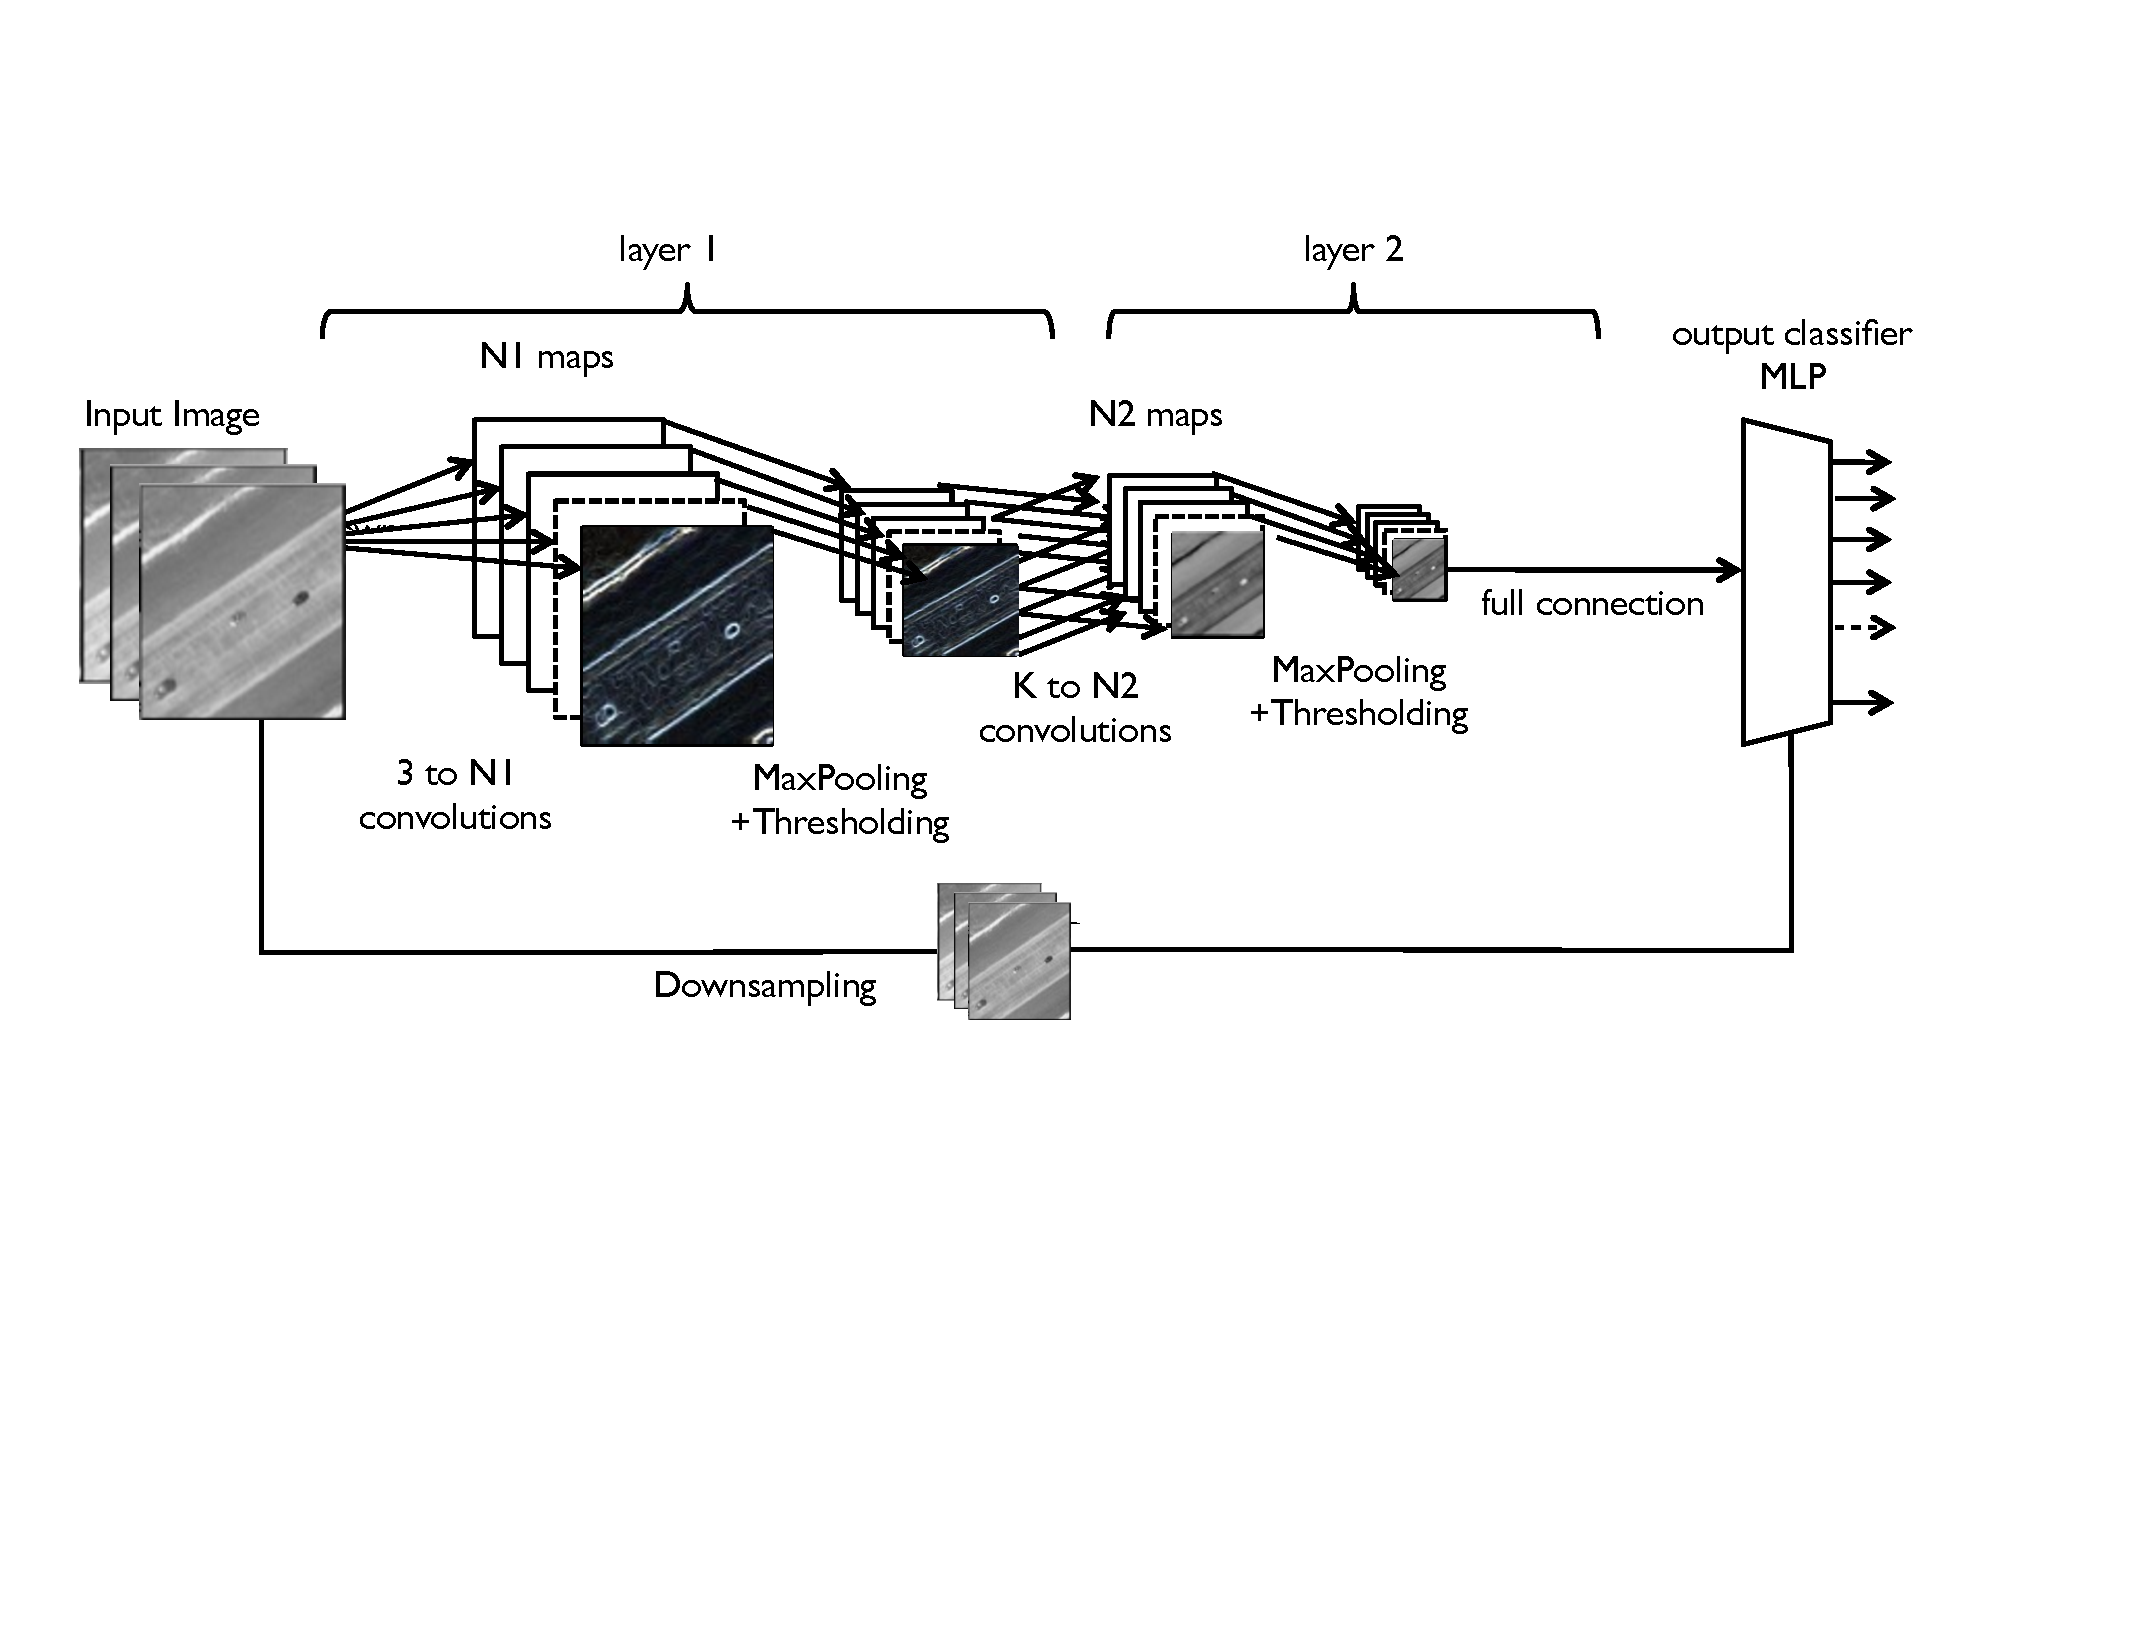
\includegraphics[width=5in]{fig-netarch.pdf}
\caption{Architecture of the CL network used in this paper: a 2 layer convolutional network with color bypass.}
\label{fig-netarch}
\end{figure}


The layers in the clustering learning network used the following sequence of operations:
\begin{enumerate}
\item Spatial Convolution module: performing convolutions on images with the learned CL filters: $yc_i=\sum_i{k_{ij}\ast x_i}$, where $\ast$ is the 2D discrete convolution operator.
\item Spatial Max Pooling module: $yp_i = max_{n \times n}(yc_{ij})$ with $n =  2$ in this work.
\item Threshold nonlinearity: $ynl_i = 0$ if $yp_i <= 0$, $ynl_i = yp_i$ if $yp_i > 0$
\end{enumerate}

All networks used 32 filters on the first layer, and 512 filters on the second layer. We use k-means clustering algorithm (we refer to this step as \textit{Clustering Learning algorithm}) to learn a set of 32 filters in the first layer, and 512 filters in the second layer. The techniques and scripts are general and can quickly modified to learn any number of filters. The filter sizes on both layers was set to 5 x 5 pixels. More information have been published in paper \cite {culurciello2013clustering}. After the first convolution, 32 filters produced 32 feature maps each size 28x28. Dimension of the feature maps decreased by 2x2 pooling with a stride of 2 pixels. We used max pooling layers because they performed better than average and gaussian-masked averages with L-2 modules. Also max pooling is a bio-inspired approach to reducing the dimensionality of the data at each layer \cite{lampl2004intracellular}. The output became 32x14x14 pixels. In the second layer, 512 filters produced output of 512x10x10 feature maps which then max pooled again and the size became 512x5x5. 
We also subsampled the RGB data by 4x4 Subsampling module with a stride of 4 pixels which gave 3x8x8 pixels.  We then concatenated the subsampled RGB data with the output of the deep network into a final vector. This final vector was then passed to a 2-layer MLP classifier. The final classifier was fixed to 128 hidden units and 10 output classes for both CIFAR and SVHN.

%Clustering learning networks used the connection matrix technique CL-connex, with receptive fields of size 32 and groups of features of size 2 and 4. The CNN networks used a fully connected input to 1st, and 1st to 2nd layer. 

 %, 2 classes for the INRIA datasets.



\subsection{Connections architecture}
????

%For the INRIA person dataset, we used a 3-layer network of size 32, 64, 128 filters in each convolutional layer.
%We experimented with SLAC connections \cite{coates2012emergence}. In this case we used 4x more features than the numbers given above as beginning features, and then we decreased them to the same size of 32,64 in each respective layer. After the Convolution modules we added a SpatialMaxMap module to compute the groups and reduce the feature numbers. Unfortunately SLAC did not give us any advantage because of the small number of features used, so we removed it from our workflow.



\subsection{Similarity of features?}
%Fig. \ref{fig-filters123} shows an example of the filters learned in all three layer of the INRIA person network trained with CL-connex.



%\begin{figure}
%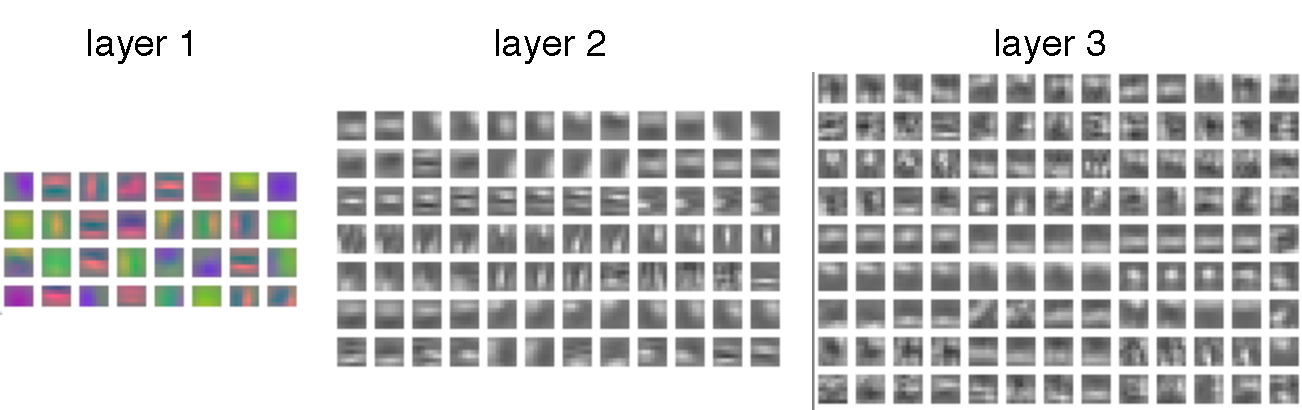
\includegraphics[width=5in]{fig-filters123.pdf}
%\caption{Filters learned with Clustering Learning and CL-Connex, for layer 1, 2, 3 respectively. These examples are from the INRIA dataset network.}
%\label{fig-filters123}
%\end{figure}


%Larger network:
%This network can be executed in real-time with accelerated hardware [neuflow]



\section{Results}
\label{sec-results}

In Fig. \ref{fig-results1} we present the results of our test on the CIFAR10 and SVHN datasets. We compared accuracy in the test-set between our CL network and a standard convolutional neural network (CNN). We report learning rates per epochs to visualize converge speed and overfitting issues.


\begin {table}
%\begin{wraptable}{r}{5cm}
\parbox{.5\linewidth}{
\caption{Results on CIFAR-10}
\label{resuts-cifar10}
\begin{center}
\begin{tabular}{ll}
\multicolumn{1}{c}{\bf Architecture}  &\multicolumn{1}{c}{\bf Accuracy}
\\ \hline \\
1 layer (32 filters)                            & $68.8\%$\\
2 layer (Fanin=1)                            &$72.8\%$ \\
2 layer (Fanin=2, random)            &$72.4\%$ \\
2 layer (Fanin=2, learned)            &$73.2\%$\\
2 layer (Fanin=32)                          &$67.0\%$\\
\\ \hline \\
CNN 1 layer                                    &$?\%$\\
CNN 2 layer                                    &$?\%$\\
\end{tabular}
\end{center}
}
%\end{wraptable}
\parbox{.5\linewidth}{
%\begin{wraptable}{r}{5cm}
\caption{Results on SVHN}
\label{resuts-svhn}
\begin{center}
\begin{tabular}{ll}
\multicolumn{1}{c}{\bf Architecture}  &\multicolumn{1}{c}{\bf Accuracy}
\\ \hline \\
1 layer (32 filters)                          & $85.7\%$\\
2 layer (Fanin=1)                           &$87.6\%$ \\
2 layer (Fanin=2, random)           &$?\%$ \\
2 layer (Fanin=2, learned)           &$?\%$\\
2 layer (Fanin=32)                        &$?\%$\\
\\ \hline \\
CNN 1 layer                                   &$?\%$\\
CNN 2 layer                                   &$?\%$\\
\end{tabular}
\end{center}
}
\end{table}
%\end{wraptable}




As one can see Fig. \ref{fig-results1}, our CL network performs very closely to the accuracy of the CNN. The CNN is always slightly better, since it uses global optimization techniques based on stochastic gradient descent (SGD) to adapt to both the signal and the noise. 

Training the CNN takes $\sim 2$ hours on our test computer with a quad core Intel i7. Training of the CL network takes $\sim 4$ minutes.
The two convolutional layers CL network are trained unsupervised using Cl on the train set for CIFAR10 and SVHN respectively. IThese layers can also be also trained with another set of natural images (a video of driving taken from YouTube), with only a slight loss of performance of $\sim 2\%$. 

Notice also that the test accuracy curves per epoch of the CL network do not overfit. Rather, they saturate to a constant average value. CL network cannot overfit by design, since they perform averages on the train-set. Because of the averaging intrinsic to the algorithms of CL, the network cannot learn specific examples of the dataset and thus overfit in the test data.


\section{Discussion}
\label{sec-disc}

We presented results on clustering learning algorithms for general-purpose vision system. These algorithms can be used to train multi-layer feed-forward neural networks from videos in minutes. We show results on ...


EUGE first draft:

In this paper we use data whitening to be able to report state-of-the-art accuracy, as done in recent work\cite{coates_analysis_2011,coates_analysis_2011,coates2012emergence,coates2012learning}. Another technique that approximate whitening used in deep network is local contrast normalization (LCN). LCN can be done on an input stream one image at a time, and does not require a history of previous frames or a dataset. On the other hand whitening requires a fixed dataset to be able to push each dimension to the largest signal-to-noise ratio. Also whitening requires computing a covariance matrix the size of convolutional patches square for all patches used in the clustering learning algorithm and also on the entire dataset. This step could be performed in parallel to inference on a set of past input frames to compute the whitening matrices, and thus adapt to environment changes. But LCN is more efficient because it does not require training on a dataset. For this reason we recommend the use of LCN in real-time applications and whitening to fixed-dataset applications that might not need to perform in real-time.

%\section{TODO}
%


\subsubsection*{Acknowledgments}
We are especially grateful to the the Torch7 developing team, in particular Ronan Collobert, who first developed this great, easy and efficient tool, Clement Farabet, Koray Kavukcuoglu, Leon Bottou. We could not have done any of this work without standing on these giants shoulders. We also thank Soumith Chintala for his help with Torch and the nice discussions.

\bibliography{clustering}
\bibliographystyle{unsrt}



\end{document}
